%!TEX root = ../thesis.tex
\begin{summarycontributions}
\cbstart
Some of the material presented in this chapter is based on joint work with Simon Lacoste-Julien and Zoubin Ghahramani, and has been published as part of \citep{Lacoste2011}.

In \citep{Lacoste2011}, two alternative approaches to approximate Bayesian computation are presented, both motivated by decision theory. The first approach sidesteps approximate inference and employs the loss-EM algorithm to perform approximate Bayesian decision theory. This approach was primarily developed by SLJ and therefore it is not presented here. FH contributed mainly to the development of the second approach, which explicitly performs approximate inference, but takes losses into acount. This chapter presents a framework called loss-calibrated approximate inference, which is based on this second approach. The main result of this chapter is connecting the loss-calibrated approximate inference framework to scoring rule-based divergences, which is original contribution by FH. Figure \ref{fig:toy}, originally created by FH, is taken from \citep{Lacoste2011} as published, with the consent of co-authors.
\cbend	
\end{summarycontributions}

% #### ##    ## ######## ########   #######  ########  ##     ##  ######  ######## ####  #######  ##    ## 
%  ##  ###   ##    ##    ##     ## ##     ## ##     ## ##     ## ##    ##    ##     ##  ##     ## ###   ## 
%  ##  ####  ##    ##    ##     ## ##     ## ##     ## ##     ## ##          ##     ##  ##     ## ####  ## 
%  ##  ## ## ##    ##    ########  ##     ## ##     ## ##     ## ##          ##     ##  ##     ## ## ## ## 
%  ##  ##  ####    ##    ##   ##   ##     ## ##     ## ##     ## ##          ##     ##  ##     ## ##  #### 
%  ##  ##   ###    ##    ##    ##  ##     ## ##     ## ##     ## ##    ##    ##     ##  ##     ## ##   ### 
% #### ##    ##    ##    ##     ##  #######  ########   #######   ######     ##    ####  #######  ##    ## 

\section{Introduction}

In Bayesian statistics, we model observed data $\data$ by introducing latent parameters $\param$, and inferring their posterior via Bayes' rule
%
\begin{equation}
	p(\param\vert\data) = \frac{p(\data\vert\param) p(\param)}{\int p(\data\vert\param) p(\param) d\param}.
\end{equation}
%
The likelihood $p(\data\vert\param)$ describes how data is related to the parameters $\param$, and $p(\param)$ is a prior distribution which captures one's a priori expectations about what the value of $\param$ may be. The posterior distribution $p_\data = p(\param\vert\data)$ captures all statistically relevant information that the data $\data$ provides about $\param$, and it is therefore of central importance.

\cbstart
The marginal likelihood, also called the model evidence $Z = \int p(\data\vert\param) p(\param) d\param$ is also of interest. In Bayesian model selection is often used to quantify how well a Bayesian model -- the combination of likelihood and prior -- fit the data. Or, when the model involves additional parameters or hyper-parameters, it is common practice to learn their values by maximising model evidence $Z$ \citep[see \eg][Chapter 5]{Rasmussen2006}. In the Bayesian paradigm, however, using the model evidence to fit hyperparameters is considered a short-cut. In a fully Bayesian approach, all unknown parameters should be modelled probabilistically via prior distributions, and their posterior distribution should be inferred via Bayes' rule. In this chapter I assume that full Bayesian inference is carried out, in other words, that the parameter $\param$ encapsulates all unknown parameters and hyper-parameters whose values we wish to infer.
\cbend

In practically interesting Bayesian models, the posterior distribution and model evidence are often computationally intractable to obtain and therefore one has to resort to approximations. The process of finding an approximate posterior distribution based on data is known as \emph{approximate Bayesian inference}. The most popular classes of methods for approximate inference are variational inference and Markov chain Monte Carlo.

Variational inference replaces the posterior by a computationally convenient distribution $q$. It operates by minimising an objective function that expresses divergence between the true posterior $p_\data$ and the approximation $q$. Most existing work on approximate inference focused on minimising a variant of the Kullback-Leibler divergence (Eqn.\ \eqref{eqn:KL_divergence}). The KL divergence allows for computationally efficient rearrangement of terms and makes local message-passing style computations possible \citep{Minka2001,Winn2006}.

As we have seen in previous chapters, the KL divergence is only one in a large class of Bregman divergences based on proper scoring rules, all of which could be used for approximate inference. In this chapter, I devise a framework called loss-calibrated approximate inference, which is based on minimising Bregman divergences related to Bayesian decision problems as described in section \ref{sec:loss_scoring_rule}. I will argue that when solving a decision problem but exact Bayesian inference is infeasibe, approximations based on the KL divergence are sub-optimal as they are ignorant of the structure of losses. In section \ref{sec:toy} I illustrate this argument through a toy example of performing approximate inference in a power plant, where losses incurred for incorrect decisions are highly asymmetric.

This chapter describes a theoretical framework for approximate Bayesian inference using general Bregman divergences, but gives no constructive guidance on the implementation of practical algorithms. In the next chapter I will focus on two algorithms, kernel herding and sequential Bayesian quadrature. I will show that these algorithms are closely related, and can be understood as approximate inference methods using the maximum mean discrepancy from Eqn.\ \eqref{eqn:rkhs-mmd-lastline} instead of the KL divergence.

% ######## ########     ###    ##     ## ######## ##      ##  #######  ########  ##    ## 
% ##       ##     ##   ## ##   ###   ### ##       ##  ##  ## ##     ## ##     ## ##   ##  
% ##       ##     ##  ##   ##  #### #### ##       ##  ##  ## ##     ## ##     ## ##  ##   
% ######   ########  ##     ## ## ### ## ######   ##  ##  ## ##     ## ########  #####    
% ##       ##   ##   ######### ##     ## ##       ##  ##  ## ##     ## ##   ##   ##  ##   
% ##       ##    ##  ##     ## ##     ## ##       ##  ##  ## ##     ## ##    ##  ##   ##  
% ##       ##     ## ##     ## ##     ## ########  ###  ###   #######  ##     ## ##    ## 

\section{Approximate inference\label{sec:losscalibrated}}

In many practically relevant cases computing the Bayesian posterior is not analytically tractable. This is predominantly due to the fact that the integral defining the marginal likelihood $\int p(\dataset\vert\param)p(\param)d\param$ cannot be computed in closed form, and therefore the posterior is only known up to a multiplicative constant. It is usual practice to approximate the intractable posterior by something simpler, a computationally convenient approximate posterior distribution $q$. The problem of finding an approximate posterior $q$ is referred to as approximate Bayesian inference.

Over the years, two dominant branches of approximate inference emerged. The first branch, that we can call parametric approximation, includes variational inference, mean-field estimation, Laplace approximation and expectation propagation. The common theme in these techniques is that the complicated posterior is replaced by an approximate distribution chosen from a particular parametric family, usually an exponential family \citep{Wainwright2008}. These methods differ in the objective functions they minimise, which measure discrepancy between the target posterior distribution $p_\data$ and the approximation $q$.

\subsection{Overview of variational methods and expectation propagation}

Variational methods to approximate inference find the optimal approximation $q^{*}$ to the posterior by maximising a lower bound to the marginal likelihood as follows.
%
\begin{align}
	\log p(\dataset) &= \log \int p(\dataset\vert\param)p(\param) d\param\\
		&=\log \int \frac{p(\dataset\vert\param)p(\param)}{q(\param)}q(\param) d\param\\
		&\geq \int \log \frac{p(\dataset\vert\param)p(\param)}{q(\param)} q(\param) d\param\\
		&= \log p(\dataset) - \KL{q}{p_{\dataset}}.      \label{eqn:variational_lower_bound}
\end{align}

Maximising this lower bound amounts to minimising the Kullback-Leibler divergence $\KL{q}{p_{\dataset}}$ (Eqn.\ \eqref{eqn:KL_divergence}) between the approximate distribution $q$ and the true posterior $p_{\dataset}$. A common practice in approximate inference is to choose the approximate posterior distribution $q$ from an exponential family of distributions $\Qe$. In addition, $q$ is often such that it factorises over multivariate quantities. When these assumptions are made, the optimal solution maximising the lower bound in Eqn.\ \eqref{eqn:variational_lower_bound} can usually be expressed in closed form. If analytic solution is not available, efficient iterative algorithms based on message passing exist for finding a locally optimal solution numerically \citep{Winn2006}.

The KL divergence is non-symmetric, therefore the order of its arguments matter. Variational methods minimise $\KL{q}{p_{\dataset}}$, that is with the approximate distribution being the first argument. Computationally, this is highly convenient as computing the divergence in this direction requires an expectation only over $q$, which is assumed simpler than the real posterior $p_{\dataset}$.

On the other hand, the scoring rule interpretation in Chapter \ref{sec:scoring_rules} suggests that the \emph{right} and theoretically well motivated way to use the divergence would be $\KL{p_{\dataset}}{q}$. This has been pointed out previously in \citep{Csato2002,Minka2001} and by several other authors. This does not mean that variational inference cannot work, it just means that when performing variational inference, we loose the convenient intuitive interpretation of KL divergence as Bregman divergence under the logarithmic loss.

Several approaches therefore tried to fix this conceptual issue, and minimise KL divergence in the opposite direction. This is technically challenging, as computing the divergence $\divergence{\score}{p_{\dataset}}{q}$ always involves computing an integral over the posterior $p_{\dataset}$, which is normally intractable. Furthermore, the convenient variational lower bound in Eqn.\ \ref{eqn:variational_lower_bound} only holds for $\divergence{\score}{q}{p_{\dataset}}$ and not for $\divergence{\score}{p_{\dataset}}{q}$.

Assumed density filtering, and its generalisation, expectation propagation (EP) try to approximate the ideal method of minimising $\KL{p_{\dataset}}{q}$ in the following way \citep{Minka2001thesis}. EP assumes the posterior can be written as a product of factors as such: 
%
\begin{equation}
	p_{\dataset}(\param) = \frac{1}{Z} \prod t_i(\param).
\end{equation}

The terms $t_i$ are assumed simple, and in most cases depend only on a few components of the multivariate parameter vector $\param$. What makes the posterior intractable is the normalisation constant $Z$, computing which would involve a very expensive integral. Expectation propagation approximates the posterior by substituting approximate factors $\tilde{t}_i$ for original factors $t_i$, in such a way that the product of approximate factors
%
\begin{equation}
	q(\param) = \prod \tilde{t}_i(\param)
\end{equation}
%
is tractable. The approximate factors are improved one-by-one using the following objective function:
%
\begin{equation}
	\tilde{t}_i^{new} = \argmin_{t \in \Qe} \KL{\underbrace{\frac{1}{\int q(\param)\frac{t_i(\param)}{\tilde{t}_i(\param)} d\param}q(\param)\frac{t_i(\param)}{\tilde{t}_i(\param)}}_{\tilde{q}}}{q(\param)\frac{t(\param)}{t_i(\param)}}. \label{eqn:expectation_propagation}
\end{equation}

Essentially, in each iteration the algorithm replaces one of the approximate factors in the approximate posterior $q$ with the real factor to construct a one-step-closer-to-exact approximation to the posterior $\tilde{q}$. Then it uses this $\tilde{q}$ as the target distribution and computes a new approximation by minimising KL divergence. This step is repeated until convergence, that is until no approximate factors can be further improved by the KL divergence metric. Since convergence of this algorithm is not guaranteed, alternative optimisation techniques with provable convergence guarantees have been proposed \citep{Seeger10}.

In expectation-propagation, the KL divergence is used in the right direction that is well motivated by the theory of scoring rules and Bregman divergences. However, instead of minimising the divergence from the true posterior, EP uses the moving target $\tilde{q}$. Expectation propagation is known to perform well in a variety of graphical models, most famously in Gaussian process classification \citep{Nickisch2008}. It exploits convenient analytic properties of the logarithmic loss and the KL divergence, which make computing the expressions in Eqn.\ \eqref{eqn:expectation_propagation} possible. Therefore the method does not readily generalise to other scoring rules or divergences.

\section{Bayesian decision theory}

Although often overlooked, the main theoretical motivations for the Bayesian paradigm are rooted in Bayesian decision theory~\citep{berger85decision}, which provides a well-defined theoretical framework for rational decision making under uncertainty about a hidden parameter $\param$. Approximate inference is concerned with approximating the posterior, but often ignores the fact that the posterior is then used in a wider context to make optimal decisions. In this section I review the theory of Bayesian decisions, and then devise a framework for addressing questions that arise when using approximate inference in the context of optimal decision making.

The ingredients of Bayesian decision theory are \citep[][Chapter 2]{robert01choice},\citep[][Chapter 1]{berger85decision}):
\vspace{-.3cm}
\begin{itemize}
  \item a loss $\loss(\param,\action)$ which quantifies the cost of taking action $\action \in \actionset$ when the world state is $\param \in \Theta$; %\footnote{Note that $\param$ is not assumed to be finite dimensional; in the most general setting, it could fully specify an arbitrary distribution over $\mathcal{O}$.};
  \item an observation model $p(\dataset|\param)$ which gives the probability of observing some data or dataset $\dataset \in \mathcal{O}$ assuming that the world state is $\param$;
  \item a prior belief $p(\param)$ over world states.
\end{itemize}

The loss $\loss$ describes the decision task that we are interested in, whereas the observation model and the prior represent our beliefs about the world. Given these components, the ultimate objective for evaluating a possible action $\action$ after observing $\dataset$ is the \emph{expected posterior loss} (also called the \emph{posterior risk}~\citep{schervish95theory}):
%
\begin{equation}
	\risk_{p_\dataset}(\action) \defeq \int_\Theta \loss(\param, a) \, p(\param|\dataset) d\param.
\end{equation}
%
In the Bayesian framework, the optimal action $\action_{p_\dataset}$ is the one that minimises $\risk_{p_\dataset}$:
%
\begin{equation}
	\action_{p_\dataset} = \argmin_{a} \risk_{p_\dataset}(\action).
\end{equation}

In this framework, Bayesian decision making decomposes into two consecutive steps of computation. First, a posterior $p_\dataset$ is inferred from observed data $\dataset$. Then, the optimal action is selected by minimising risk under this posterior. Crucially, the first step is independent of losses, the posterior can be computed irrespective of how the loss $\loss$ is defined. In fact, once we have computed the posterior, the same distribution can be used to solve different decision problems with different losses involved. This independent breakdown of computation is what makes the posterior distribution such an important object in Bayesian statistics.

But when the posterior is intractable to compute and approximations are needed - as it is the case most of the time - additional questions arise. Is this two-step breakdown of computations to inference and then risk minimisation still a sensible thing to do? How should we decide what approximate inference method to use? Can we still re-use the same approximate posterior with different loss functions just as we can if no approximations are needed. Is the choice of approximate inference technique independent of the loss function? This chapter introduces loss-calibrated approximate Bayesian inference as a theoretical framework for addressing these questions.

\section{The loss-calibrated approximate inference framework}

When performing approximate inference in the context of Bayesian decision making, one usually treats the approximate posterior $q$ as if it was the true posterior and chooses the action that minimises what we will call the \emph{$q$-risk}:
%
\begin{equation} \label{e:q-risk}
	\mathcal{R}_q(h) \defeq \int_\Theta q(\param) L(\param,h) d\param,
\end{equation}
%
obtaining a \emph{$q$-optimal} action $\action_q$:
%
\begin{equation}
	\action_q \defeq \argmin_{\action \in \actionset} \mathcal{R}_q(\action).
\end{equation}

In this framework, we will assume that computing exactly the $q$-optimal action $\action_q$ for $q \in \mathcal{Q}$ is tractable, and focus on the problem of choosing a suitable $q$ to approximate the posterior $p_\dataset$.

Surely, unless $q$ matches the posterior $p_\dataset$ exactly, the $q$-optimal action $\action_q$ will not necessarily be optimal under $p_\dataset$. The true posterior risk $\mathcal{R}_{p_\dataset}(\action_q)$ of $a_q$ is going to be higher than the Bayes risk $\mathcal{R}_{p_\dataset}(\action_{p_\dataset})$. A sensible objective therefore is to minimise the excess risk incurred because we use an approximate posterior. An optimal approximate posterior $q \in \mathcal{Q}$ is clearly:
%
\begin{equation}
	q_\mathrm{opt} = \argmin_{q \in \mathcal{Q}} \mathcal{R}_{p_\dataset}(\action_q).
\end{equation}

In the case where $p_\dataset\in\mathcal{Q}$, that is, when the true posterior is a member of the approximating family, $p_\dataset$ is obviously optimal according to this criterion. We could interpret the above criterion as minimising the following asymmetric divergence measure between distributions:
%
\begin{equation} \label{e:d_L}
	\divergence{\loss}{p_\dataset}{q} \defeq \mathcal{R}_{p_{\dataset}}(\action_q) - \mathcal{R}_{p_\dataset}(\action_{p_\dataset}),
\end{equation}
%
which is the same as the Bregman divergence defined in section \ref{sec:loss_scoring_rule}.

As mentioned in Chapter \ref{sec:scoring_rules}, the divergences defined via Bayesian decision problems are equivalent to Bregman divergences defined via proper scoring rules. One can therefore express the goal of loss-calibrated approximate inference as minimising a Bregman divergence for an arbitrary scoring rule over the posterior:
%
\begin{equation}
	\argmin_{q \in \mathcal{Q}} \divergence{S}{p_{\dataset}}{q}.
\end{equation}

Interestingly, the Kullback-Leibler divergence $\KL{p}{q}$ is a special case of $d_\loss$, hence the algorithms developed for (approximately) minimising  $\KL{p_\dataset}{q}$ are a special case of this ``loss-calibrated'' framework. The loss $\loss$ in this case can be interpreted as the description length of the true underlying parameter $\param$ based on optimal coding under $q$ (see section \ref{sec:loss_scoring_rule}).

But this begs the natural question of whether minimising $d_\loss$ for a particular loss $\loss$ provides optimal performance under other losses. If this was the case, then existing algorithms for KL-divergence optimisation would be sufficient to solve general loss-calibrated approximate inference problems. Unfortunately, as I will illustrate in the following section, the optimal solution under one scoring rule can lead to suboptimal performance for another loss function. This motivates future research into practical approximate inference algorithms that minimise general Bregman divergences.

\section{Illustration of the framework \label{sec:toy}}

\begin{figure}
\centering
\begin{tikzpicture}
	\node at (0.1in,0.1in) [anchor = south west] {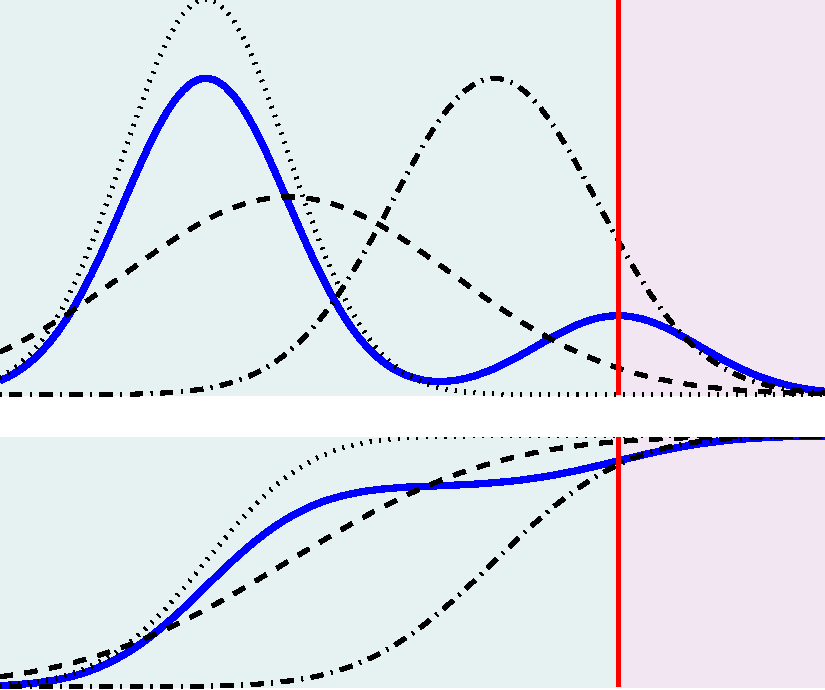
\includegraphics[width=3in]{figs/lossBayes/toy_figure.pdf}};
	\node at (1.6in,0in) {$\theta$ (plant temperature)};
	\node at (2.5in,0in) {$T_\mathrm{crit}$};
	\node [rotate = 90] at (0in,0.6in) {$\mathbb{P}[T<\theta]$};
	\node [rotate = 90] at (0in,2in) {$p(\theta)$};
\end{tikzpicture}
 \caption[Illustrating of approximate inference in a loss-critical toy example]{\textbf{Top:} Real bimodal posterior \emph{(blue)} and three Gaussian approximations obtained by minimising  $\KL{q}{p}$ \emph{($q_1$, dotted)}, $\KL{p}{q}$ \emph{($q_2$, dashed)} or $\divergence{\loss}{p}{q}$ \emph{($q_3$, dash-dotted)} in the power plant example. \textbf{Bottom:} Cumulative distribution functions for the posterior and the three approximate distributions. Observe how the KL-divergence based approximations overshoot the probability that the temperature is below the critical level.}  \label{fig:toy}
\end{figure}

To illustrate the role and behaviour of approximate inference in a Bayesian decision problem consider the following simple problem. Suppose that we control a nuclear power-plant which has an unknown temperature $\theta$ that we model with Bayesian inference based on some measurements $\data$.

The plant is in danger of over-heating, and as the operator, we can take two actions: either shut it down or keep it running. Keeping it running while the temperature is above a critical threshold $T_\mathrm{crit}$ will cause a nuclear meltdown, incurring a large loss $L(\theta>T_\mathrm{crit},\mbox{`on'})$. On the other hand, shutting down the power plant incurs a moderate loss $L(\mbox{`off'})$, irrespective of the temperature. 
%Given our posterior $p_\dataset$ and the losses, we want to compute the Bayes-optimal action that minimizes the posterior risk. 
Suppose that our current observations yielded a complicated multi-modal posterior $p_\dataset(\theta)$ (\ref{fig:toy}, solid curve) that we do not have computational resources to represent. Thus we chose to approximate it with a simple Gaussian distribution.

Now consider how various approaches to approximate inference would perform in terms of their Bayesian posterior risk. Minimising $\KL{q}{p_\dataset}$, as in variational inference, yields candidate $q_1$ which concentrates around the largest mode, ignoring entirely the second small mode around the critical temperature \ref{fig:toy}, dotted curve). Minimising $\KL{p_\dataset}{q}$ gives a more global approximation: $q_2$ matches moments of the posterior, but still underestimates the probability of the temperature being above $T_\mathrm{crit}$, thereby leading to a suboptimal decision \ref{fig:toy}, dashed curve).

$q_3$ is one of the minimisers of $\divergence{\loss}{p_\dataset}{q}$ in this setting, that results in the same decision as $p_\dataset$ \ref{fig:toy}, dash-dotted curve). Note that $q_3$ does not model all aspects of the posterior, but it estimates the Bayes-decision well. Because there are only two possible actions in this setup, the set $\mathcal{Q}$ is split in only two halves by the function $\divergence{\loss}{p_\dataset}{q}$: those which would result in the same action as $p_{\dataset}$, and those which would result in the opposite. Consequently, there are infinitely many $q_\mathrm{opt}$s that are equivalent in terms of the divergence.

This simple example highlights some features of the loss-calibrated framework. First of all, it is clear, that even in a simple example the choice of approximate inference methods matters, and has a great influence on risks and the final decisions made. In this case minimising $\KL{p_\dataset}{q}$ yielded a solution superior to minimising the variational criterion $\KL{q}{p_\dataset}$, but we could just as well construct another example, where it is the other way around. Even though minimising $\KL{p_\dataset}{q}$ is an instance of loss-calibrated inference, in the context of this decision problem it is an inappropriate choice, because the assumed losses are now different.

In \citep{Lacoste2011} we give further examples of loss-calibrated Bayesian inference problems where minimising KL divergence leads to suboptimal performance. This motivates further research into approximate inference based on various Bregman divergences that differ from the KL divergence. Unfortunately, this is a hard problem in general, because evaluating the divergence requires taking expectations over the posterior, which is often impossible. In fact the very reason for approximating the posterior is to be able to approximate expectations over it.

In the following chapter I will examine kernel herding, an algorithm that can be thought of as minimising maximum mean discrepancy, and thus, an instance of loss-calibrated inference.

\section{Loss-calibrated quasi-Monte Carlo}

A popular alternative to parametric approximation schemes, such as variational inference and expectation propagation are Monte Carlo methods \citep[see \eg][]{Murray2007}.

Monte Carlo methods produce random samples $\param_n$ from the posterior distribution $p_\dataset$ and then approximate relevant integrals by taking the empirical mean over these samples:
%
\begin{equation}
	\expect{\param \sim p_{\dataset}} f(\param) \approx \frac{1}{N} \sum_{n = 1}^{N} f(\param_N).
\end{equation}

Subject to smoothness conditions, this non-deterministic estimate of any integral converges at a rate $\mathcal{O}(\frac{1}{\sqrt{N}})$, where $N$ is the number of samples. This convergence is guaranteed by the law of large numbers. An appealing property of Monte Carlo methods is that in theory an arbitrarily precise estimate can be obtained by just increasing the number of samples. In this sense, Monte Carlo approximation is non-parametric: the number of parameters that describe the approximate distribution is not fixed ahead of time, and can be arbitrarily large.

When exact sampling from $p_\dataset$ is impossible or impractical, Markov chain Monte Carlo (MCMC) methods are often used. MCMC methods only require knowing the target distribution up to a constant factor. Practically this means that even if the normalisation constant of the posterior is intractable, MCMC techniques can still be used to generate samples from it.

Various variants of MCMC methods can be applied to almost any problem but the convergence rate of the estimate depends on several factors and is hard to estimate \citep{CowlesCarlin96}. Typically, MCMC techniques introduce positive correlation between subsequent samples, and thus are less effective than exact Monte Carlo sampling. For an overview of various Monte Carlo techniques, see \citep{Murray2007}.

Monte Carlo methods are very general, they guarantee convergence for any measurable integral. Hence, convergence is also guaranteed in the KL divergence sense, and as the posterior risk is expressed as an integral, they also ensure convergence in $\divergence{\loss}{\cdot}{\cdot}$ for any loss function $\ell$. However, the rate of convergence cannot be fine-tuned to a particular divergence measure. One might hope that if the loss function $\loss$ is known ahead of time, a faster convergence rate can be achieved, maybe at the cost of slowing down convergence on integrals that are irrelevant to the decision problem.

\subsection{Quasi-Monte Carlo approaches}

The focus of the following chapter is an example of quasi-Monte Carlo methods that -- instead of sampling randomly -- produce a set of pseudo-samples in a deterministic fashion. These methods operate by directly minimising some sort of discrepancy between the empirical distribution of pseudo-samples and the target distribution. Whenever these methods are applicable, they achieve convergence rates superior to the $\mathcal{O}(\nicefrac{1}{\sqrt{N}})$ rate typical of random sampling.

The most commonly used quasi-Monte Carlo methods include Sobol sequences \citep{Sobol1967,Sobol1998} and Halton sequences \citep{Halton1964} and modern variants thereof. A thorough, despite somewhat outdated review of these classical methods can be found in \citep{Niederreiter1992}. For a more recent account is given in \citep{Lemieux2009}.

Classical quasi-Monte-Carlo usually aims at producing low-discrepancy sequences in a unit cube that are approximately uniformly distributed. These methods often achieve faster convergence rates than traditional random Monte Carlo, and can be extended to produce pseudo-samples from arbitrary multidimensional distributions. Just like Monte Carlo, they are general-purpose sampling tools: they cannot be fine-tuned to particular decision problems we may want to use them for. Here I will introduce a loss-calibrated quasi-Monte Carlo methods, which work similarly to traditional QMC, but minimise loss-calibrated Bregman divergences instead.

Given a distribution $p\in\probmeasures{\Theta}$, Quasi-Monte-Carlo methods produce a sequence of pseudo-samples $\param_1,\ldots,\param_N$. They can be interpreted as a special case of approximate inference, where the approximating family is the family of empirical distributions parametrised by the location of pseudo-samples:
%
\begin{equation}
	q(\param ; \param_1,\ldots,\param_N) = \frac{1}{N} \sum_{n=1}^{N} \delta(\param - \param_n).
\end{equation}

Other variants assign weights to pseudo-samples therefore their approximating family are weighted empirical distributions
%
\begin{equation}
	q(\param ; \param_1,\ldots,\param_N,w_1,\ldots,w_N) = \sum_{n=1}^{N} w_n \delta(\param - \param_n).
\end{equation}

To find the optimal sequence of pseudo-samples, QMC methods minimise a discrepancy criterion. In loss-calibrated approximate inference the goal is to minimise the loss-calibrated divergence $d_\loss$ between the target distribution $p_\dataset$ and the approximation $q$. This criterion can applied to quasi-Monte Carlo:
%
\begin{equation}
	\{\param_1,\ldots,\param_N\}_{n=1}^{N} \leftarrow \argmin_{\{\param_1,\ldots,\param_N\}_{n=1}^{N}} \divergence{\loss}{p_\dataset}{q(\cdot ; \param_1,\ldots,\param_N)}. \label{eqn:loss_calibrated_nonsequential}
\end{equation}

It is important to note, that the above objective is not always well defined for certain Bregman divergences. For example, the KL divergence $\KL{p}{q}$ requires the approximate distribution $q$ to be absolutely continuous with respect to the target distribution $p$, which, unless the target distribution is also discrete, cannot be satisfied if $q$ is an empirical distribution. This means that the KL divergence cannot be applied as a discrepancy criterion in quasi-Monte Carlo.

The optimisation problem in Eqn.\ \ref{eqn:loss_calibrated_nonsequential} assumes that all pseudo-sample locations are optimised jointly. This is often infeasible in practice. Instead, pseudo-samples are usually generated sequentially using the myopic criterion, optimising the location of the next pseudo-sample, given the set of pseudo-samples already fixed. This gives rise to the following procedure called loss-calibrated quasi-Monte Carlo:
%
\begin{equation}
	\param_{n+1} \leftarrow \argmin_{\param \in \Theta} \divergence{\loss}{p_\dataset}{q(\cdot ; \param_1,\ldots,\param_{n},\param)}. \label{eqn:loss_calibrated_sequential}
\end{equation}

Just as loss-calibrated approximate inference in general, algorithmic implementation of loss-calibrated QMC requires the ability to evaluate certain expectations over the target distribution easily. Therefore practical applications of loss-calibrated QMC in the form presented here are limited. Nevertheless, the framework may provide useful blueprint for designing sampling algorithms that are more tailored to particular loss functions.

\section{Summary}

In this chapter I explored the role of divergences in approximate Bayesian inference. Deriving from Bayesian first principles I argued that, when Bayesian analysis is used to solve a decision problem, losses should be taken into account in approximate inference. Under these assumptions, one should minimise loss-calibrated divergence $\divergence{\loss}{\cdot}{\cdot}$ of Eqn.\ \eqref{e:d_L}. I argued that this class of divergence functionals is exactly equivalent to Bregman divergences based on proper scoring rules (see Section \ref{sec:loss_scoring_rule}). Thus, one can formulate the goal of approximate inference as minimising a Bregman divergence between the true posterior $p_{\data}$ and an approximate distribution $q$.

The most common approximate inference algorithms aim at reducing the KL divergence, a special case of Bregman divergences. I reviewed several algorithms based on KL divergences, none of which solve the problem entirely satisfactorily. Variational inference minimises KL divergence in the ``wrong'' direction; expectation propagation uses a proximate distribution in place of the true posterior. In the following chapter I focus on kernel herding and Bayesian quadrature, examples of loss-calibrated quasi-Monte Carlo that aim to minimise maximum mean discrepancy, a Bregman divergence based on the kernel score.